\documentclass[11pt,a4paper]{article}
\usepackage[UTF8,fontset=none]{ctex}
\usepackage{fontspec}
\setmainfont{DejaVu Serif}
\setsansfont{DejaVu Sans}
\setCJKmainfont{Noto Serif CJK SC}
\setCJKsansfont{Noto Sans CJK SC}
\setCJKmonofont[Extension=.otf]{FandolFang-Regular}
\usepackage[a4paper,top=18mm,bottom=19mm,left=18mm,right=18mm]{geometry}
\usepackage{graphicx,booktabs,tabularx,array}
\usepackage{amsmath,amssymb}
\usepackage{xcolor}
\usepackage{titlesec}
\usepackage{fancyhdr}
\usepackage{caption}
\usepackage{float}
\usepackage{hyperref}
\usepackage[most]{tcolorbox}
\usepackage{microtype}
\usepackage{tikz}
\usetikzlibrary{positioning,arrows.meta,calc,fit}

% Smart Cities & Location Services — P2 Cloud Sorbet
% LOCKED visual palette v1 for Experiment Report
\definecolor{Paper}{HTML}{FCFAF7}
\definecolor{Ink}{HTML}{2D3238}
\definecolor{Muted}{HTML}{70757A}
\definecolor{P1}{HTML}{D3EAF5} % light blue
\definecolor{P2}{HTML}{F5D9B8} % apricot
\definecolor{P3}{HTML}{E8C7D3} % soft rose
\definecolor{P4}{HTML}{D7D3EA} % mist violet
\definecolor{C1}{HTML}{5B9FBE} % blue accent
\definecolor{C2}{HTML}{D49757} % apricot accent
\definecolor{C3}{HTML}{B97589} % rose accent
\definecolor{C4}{HTML}{8177A8} % violet accent
\definecolor{Rule}{HTML}{DDE3E7}
\definecolor{Panel}{HTML}{FFFDFC}

% Shared palette and TikZ are loaded by the parent document.
% No evidence-specific coordinates or semantic relations belong here.
\tikzset{
  ie before/.style={draw=C1,fill=P1},
  ie user/.style={draw=C2,fill=P2},
  ie user rose/.style={draw=C3,fill=P3},
  ie after/.style={draw=C4,fill=P4},
  ie connector/.style={draw=C1,line width=.8pt,-{Latex[length=2mm]},rounded corners=2pt},
  ie note/.style={anchor=north west,align=left,text width=40mm,
    font=\sffamily\small,text=Ink,inner sep=0pt},
  ie label/.style={anchor=north west,align=left,font=\sffamily\scriptsize,
    text=Muted,inner sep=0pt}
}

% Direct embed with graphicx options, including trim={L B R T},clip.
\newcommand{\IEScreenshot}[3][]{\includegraphics[width=#3,#1]{#2}}

% Coordinates inside are normalized to the displayed (possibly cropped) image.
% (0,0) = bottom left; (1,1) = top right. Text sizes remain physical sizes.
\newenvironment{interactionevidence}[3][]{%
  \begin{tikzpicture}
  \node[anchor=south west,inner sep=0pt,outer sep=0pt] (ieimage) at (0,0)
    {\IEScreenshot[#1]{#2}{#3}};
  \begin{scope}[x={(ieimage.south east)},y={(ieimage.north west)}]
}{%
  \end{scope}
  \end{tikzpicture}%
}

\newcommand{\IEHighlight}[3][ie user]{%
  \path[#1,fill opacity=.28,draw opacity=.8,line width=.6pt,
    rounded corners=1.2pt] (#2) rectangle (#3);}
\newcommand{\IEOutline}[3][ie user]{%
  \path[#1,fill=none,line width=.8pt,rounded corners=1.2pt]
    (#2) rectangle (#3);}
\newcommand{\IEAnchor}[2]{\coordinate (#1) at (#2);}
\newcommand{\IEMarker}[3][ie user]{%
  \node[#1,circle,inner sep=1.6pt,font=\sffamily\scriptsize\bfseries,
    text=Ink] at (#2) {#3};}
\newcommand{\IECurvedArrow}[3][]{%
  \draw[ie connector,#1] (#2) to[out=-20,in=20] (#3);}
% #2 is an explicit TikZ route; endpoints are approved phrase anchors.
\newcommand{\IERoutedArrow}[2][]{\draw[ie connector,#1] #2;}
\newcommand{\IESideNote}[3][]{\node[ie note,#1] at (#2) {#3};}
\newcommand{\IEProvenance}[3][]{\node[ie label,#1] at (#2) {#3};}
\newcommand{\IEAssetLabel}[2]{\IEProvenance{#1}{Asset layer: #2}}


\pagecolor{Paper}
\color{Ink}

\hypersetup{
  colorlinks=true,
  linkcolor=C1,
  urlcolor=C1,
  citecolor=C4
}

\setlength{\parindent}{2em}
\setlength{\parskip}{0.24em}
\linespread{1.17}

\titleformat{\section}[hang]
  {\sffamily\bfseries}
  {\fontsize{26}{26}\selectfont\color{C1}\thesection}
  {0.68em}
  {\Large}

\titleformat{\subsection}
  {\sffamily\large\bfseries\color{Ink}}
  {\thesubsection}
  {0.55em}
  {}

\titlespacing*{\section}{0pt}{1.85em}{0.75em}

\pagestyle{fancy}
\fancyhf{}
\fancyhead[L]{\sffamily\small\color{Muted}SMART CITIES \& LOCATION SERVICES}
\fancyhead[R]{\sffamily\small\color{Muted}Process Report}
\fancyfoot[C]{\sffamily\small\color{Muted}\thepage}
\renewcommand{\headrulewidth}{0pt}

\captionsetup{
  font=small,
  labelfont={bf,sf,color=Ink},
  textfont={color=Ink},
  skip=5pt
}

\newtcolorbox{contextbox}{
  enhanced,
  boxrule=.45pt,
  colframe=Rule,
  colback=Panel,
  left=4mm,
  right=4mm,
  top=2.4mm,
  bottom=2.4mm,
  arc=1mm
}

\newtcolorbox{decisionbox}[1][C4]{
  enhanced,
  boxrule=.45pt,
  colframe=Rule,
  colback=Panel,
  borderline west={2.6pt}{0pt}{#1},
  left=4mm,
  right=4mm,
  top=2.4mm,
  bottom=2.4mm,
  arc=1mm
}

\newcommand{\semantic}[2]{%
  \tikz[baseline=-.6ex]
  \node[
    rounded corners=1.4pt,
    inner xsep=4pt,
    inner ysep=1.4pt,
    fill=#1!68!white,
    text=Ink,
    font=\sffamily\scriptsize\bfseries
  ]{#2};%
}

\begin{document}

% The unnumbered cover must not duplicate the following page.1 anchor.
\hypersetup{pageanchor=false}

\begin{titlepage}
\thispagestyle{empty}

\vspace*{25mm}

{\sffamily\small\color{C1}\bfseries
SMART CITIES \& LOCATION SERVICES
}\par

\vspace{5mm}

{\sffamily\fontsize{27}{32}\selectfont\bfseries
Process Report
}\par

\vspace{3mm}

{\Large
Human--AI Workflow \& Research Process
}\par

\vspace{12mm}

\noindent
\color{Rule}
\rule{\linewidth}{0.8pt}
\color{Ink}

\vspace{10mm}

\begin{tabular}{@{}>{\sffamily\color{Muted}}p{30mm}p{104mm}@{}}
报告类型
&
Process Report / AI 使用与研究过程文档
\\

内容结构
&
Workflow Construction + Experiment Decision Process
\\

视觉基线
&
P2 · Cloud Sorbet Exact
\\

核心图型
&
Editorial Board / Human Reasoning / Horizontal Candidate Tree
\\

状态
&
Design System v2.2（正式任务中必须替换为真实交互、真实证据和真实决定）
\end{tabular}

\vfill

\noindent
\color{P1}\rule{0.30\linewidth}{3.2pt}%
\color{P2}\rule{0.22\linewidth}{3.2pt}%
\color{P3}\rule{0.24\linewidth}{3.2pt}%
\color{P4}\rule{0.12\linewidth}{3.2pt}

\par
\vspace{5mm}

{\small\color{Muted}
本模板展示 Process Report 的信息结构、证据组织与视觉语言；
所有示例内容均为版式示意，不代表真实实验或真实 Human--AI 互动。
}

\end{titlepage}

\hypersetup{pageanchor=true}

\tableofcontents
\clearpage

% ============================================================
% 1. Two-layer Process Report structure
% ============================================================

\section{工作流构建与实验决策：Process Report 的双层结构}

\begin{contextbox}
\textbf{Process Report 不只记录实验方法讨论。}
正式内容包含两个互补层次：
\textbf{Workflow Construction}
说明可靠 Human--AI 研究工作流怎样一步步形成；
\textbf{Experiment Decision Process}
说明具体实验方法、参数、指标和结论怎样通过真实互动、资料与实验形成。

是否进入正式主体，不按“是不是项目管理”机械判断，
而看它是否真实改变了职责、证据链、复现方式、研究治理或正式产物结构。
\end{contextbox}

\vspace{0.7em}

\begin{center}
\begin{tikzpicture}[
  x=1cm,
  y=1cm,
  every node/.style={
    font=\sffamily\small,
    align=center
  }
]

\node[
  draw=Ink!35,
  fill=white,
  rounded corners=3pt,
  minimum width=3.8cm,
  minimum height=.95cm,
  line width=.7pt
] (p) at (0,2.1)
{Process Report};

\node[
  draw=C1!75,
  fill=white,
  rounded corners=3pt,
  minimum width=5.4cm,
  minimum height=1.0cm,
  line width=1pt
] (w) at (-4.0,.55)
{A · Workflow Construction\\工作流如何形成};

\node[
  draw=C4!75,
  fill=white,
  rounded corners=3pt,
  minimum width=5.4cm,
  minimum height=1.0cm,
  line width=1pt
] (e) at (4.0,.55)
{B · Experiment Decision Process\\实验决策如何形成};

\draw[
  -{Latex[length=2mm]},
  Ink!45,
  line width=.8pt
] (p) -- (w);

\draw[
  -{Latex[length=2mm]},
  Ink!45,
  line width=.8pt
] (p) -- (e);

\node[
  draw=Ink!22,
  fill=white,
  rounded corners=2.5pt,
  minimum width=3.2cm,
  minimum height=.82cm
] (w1) at (-6.0,-1.0)
{角色与治理\\GPT / 用户 / Codex};

\node[
  draw=Ink!22,
  fill=white,
  rounded corners=2.5pt,
  minimum width=3.2cm,
  minimum height=.82cm
] (w2) at (-2.0,-1.0)
{证据与复现\\Audit / GitHub / Evidence};

\node[
  draw=Ink!22,
  fill=white,
  rounded corners=2.5pt,
  minimum width=3.2cm,
  minimum height=.82cm
] (e1) at (2.0,-1.0)
{方法与参数\\候选 / 假设 / 指标};

\node[
  draw=Ink!22,
  fill=white,
  rounded corners=2.5pt,
  minimum width=3.2cm,
  minimum height=.82cm
] (e2) at (6.0,-1.0)
{验证与裁决\\资料 / 数据 / 实验};

\foreach \n in {w1,w2}{
  \draw[
    -{Latex[length=1.8mm]},
    C1!80,
    line width=.7pt
  ] (w) -- (\n);
}

\foreach \n in {e1,e2}{
  \draw[
    -{Latex[length=1.8mm]},
    C4!80,
    line width=.7pt
  ] (e) -- (\n);
}

\node[
  draw=C2!75,
  fill=white,
  rounded corners=3pt,
  minimum width=4.8cm,
  minimum height=.9cm,
  line width=1pt
] (u) at (-3.0,-2.7)
{用户真实判断\\发现 / 质疑 / 修改 / 否决 / 选择};

\node[
  draw=C4!75,
  fill=white,
  rounded corners=3pt,
  minimum width=4.8cm,
  minimum height=.9cm,
  line width=1pt
] (d) at (3.0,-2.7)
{证据驱动收敛\\Evidence → Decision → Confirmation};

\draw[
  -{Latex[length=2mm]},
  C2,
  line width=.9pt
] (w1.south) -- (u.north west);

\draw[
  -{Latex[length=2mm]},
  C2,
  line width=.9pt
] (e1.south) -- (u.north east);

\draw[
  -{Latex[length=2mm]},
  C4,
  line width=.9pt
] (w2.south) -- (d.north west);

\draw[
  -{Latex[length=2mm]},
  C4,
  line width=.9pt
] (e2.south) -- (d.north east);

\end{tikzpicture}
\end{center}

\begin{decisionbox}[C2]
\textbf{Brainstorm 的双重职责。}

Process Report 可以保留真实 v1 / v2 / v3 的发散、质疑、修改、淘汰和收敛：
既可以记录工作流如何形成，也可以记录实验方案如何形成。

Experiment Report 若确有技术价值，
只保留高度提炼后的最终方法设计、候选选择或评价框架，
不复制聊天过程或 Process Brainstorm。
\end{decisionbox}

% ============================================================
% 2. General process / contact sheet
% ============================================================

\clearpage

\section{一般过程：截图汇总}

\begin{contextbox}
一般过程同样保留真实截图，但在正式报告中按阶段汇总。

截图是证据主体；
文字只说明这一阶段解决了什么问题、
用户作出了什么实质判断、
形成了什么可继续推进的结果。

Workflow Construction 与 Experiment Decision Process
都可以使用 Contact Sheet；
完整原图进入 Evidence Archive。
\end{contextbox}

\begin{figure}[H]
\centering
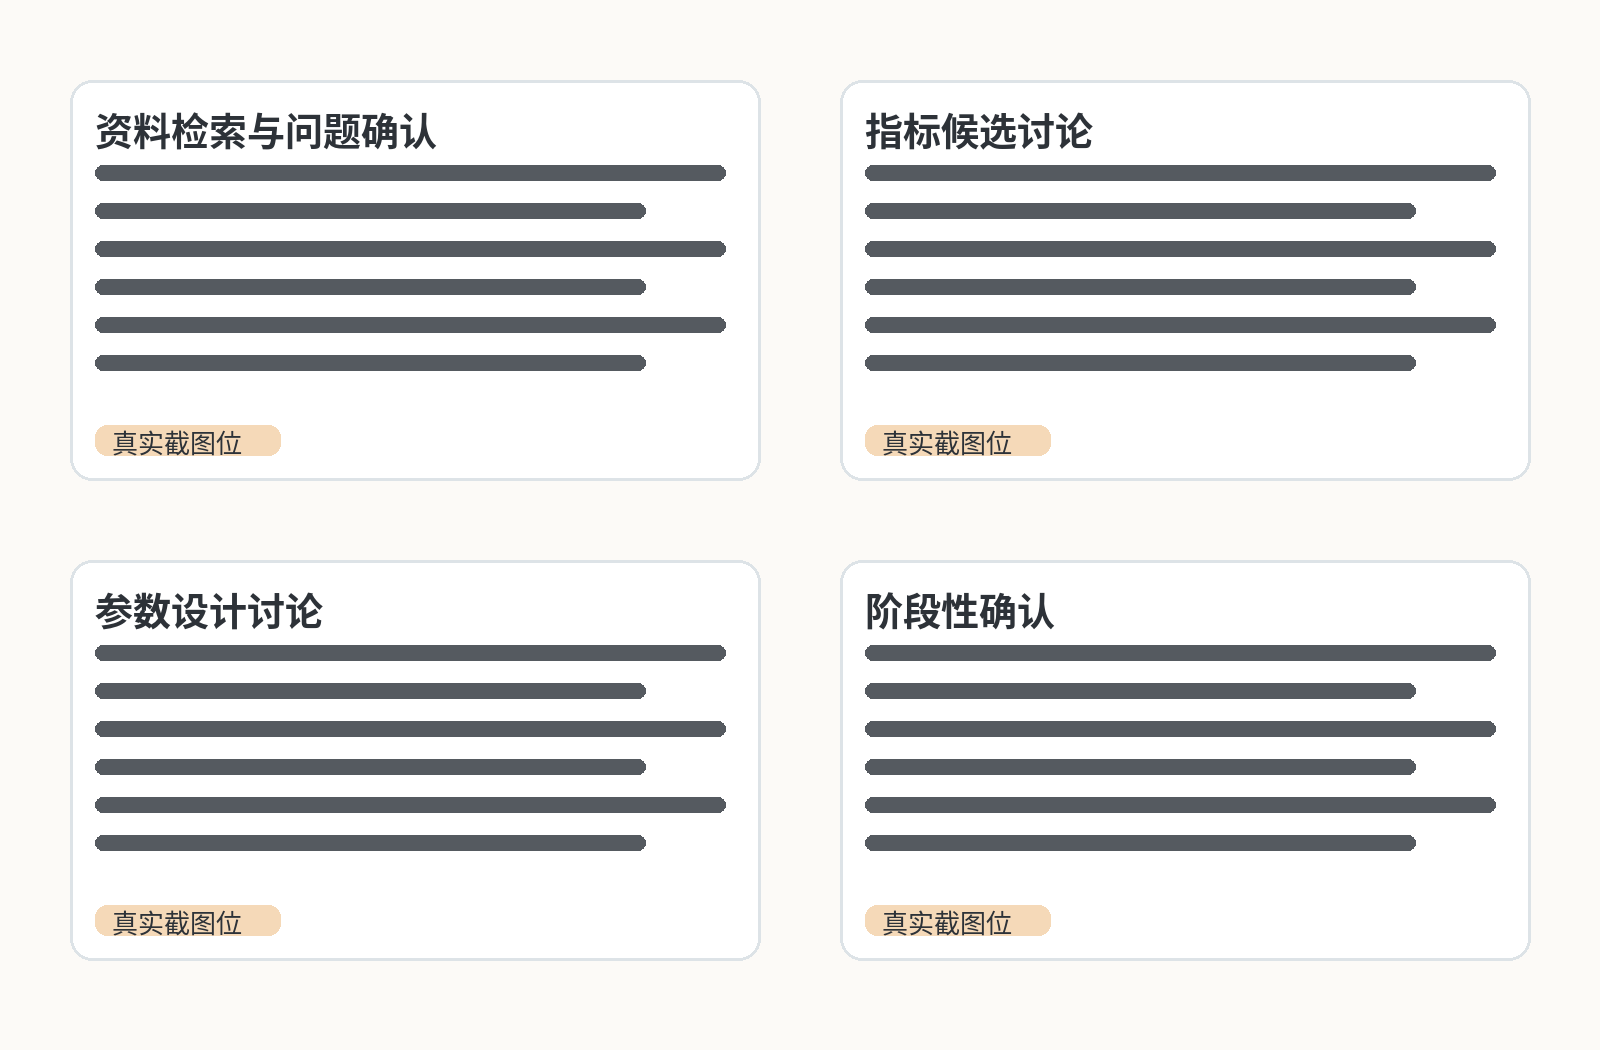
\includegraphics[
  width=.93\linewidth
]{demo-assets/contact_sheet.png}
\caption{
SYNTHETIC / TEMPLATE ONLY：一般过程汇总的版式示例。
正式版本替换为同阶段的真实 ChatGPT 网页截图。
}
\end{figure}

\begin{decisionbox}[C1]
\textbf{阶段结果示例（非实验结论）。}

资料检索、任务理解、工作流规则形成、数据理解、
指标讨论和阶段性确认均可按价值汇总；

真正改变研究工作流或实验方法的关键对话应单独展开。

缓存清理、普通路径修复和无意义 Debug
不进入正式主体。
\end{decisionbox}

% ============================================================
% Synthetic Micro Trace fixture; never treat these phrases as real evidence.
% ============================================================
\clearpage
\section{短语对应与矢量批注：模板示例}

\begin{contextbox}
\textbf{SYNTHETIC / TEMPLATE ONLY}
本页使用非聊天 UI 的合成文字样张，仅验证高清 PNG 直接嵌入、
phrase highlight、User anchor、长箭头与侧注的工程能力。
示例句及关系不代表真实用户观点、历史互动或 Evidence Lock。
正式页面必须采用 Evidence Master 批准的原图与 annotation specification。
\end{contextbox}

\vspace{3mm}
\noindent
\begin{interactionevidence}[trim={0 0 0 0},clip]{demo-assets/micro_trace_specimen.png}{110mm}
  \IEHighlight[ie before]{.079,.658}{.535,.704}
  \IEHighlight[ie user]{.079,.418}{.490,.464}
  \IEOutline[ie user]{.079,.418}{.490,.464}
  \IEHighlight[ie after]{.079,.178}{.540,.224}
  \IEAnchor{before-phrase}{.535,.68}
  \IEAnchor{user-phrase}{.490,.44}
  \IEAnchor{after-phrase}{.540,.20}
  \IEMarker{.045,.44}{1}
  \IECurvedArrow{user-phrase}{before-phrase}
  \IERoutedArrow{(user-phrase) -- (.86,.44) -- (.86,.20) -- (after-phrase)}
  \IESideNote{1.07,.74}{\textbf{① 示例动作与后续变化}\par
    合成样例中的用户要求保留短语可读性；后续示例将单页安排改为跨页。
    两条箭头只演示明确短语之间的对应，不构成真实历史证据。}
  \IEProvenance[text width=40mm]{1.07,.30}{SYNTHETIC / TEMPLATE ONLY\\
    Vector overlay: TikZ\\No Evidence Lock}
  \IEAssetLabel{0,-.04}{synthetic PNG + vector annotation}
\end{interactionevidence}

\vspace{5mm}
\noindent\small
样张以 300 dpi 原生栅格化，在 110 mm 宽度直接显示，约 300 effective PPI。
正式截图须分别记录 raw/crop 像素与最终尺寸；PDF 的 200-dpi 检查渲染不能提升原图清晰度。
\normalsize

% ============================================================
% 3. Multi-page core interaction evidence
% ============================================================

\clearpage

\section{核心交互：连续多页证据（1/3）}

\begin{contextbox}
\textbf{SYNTHETIC / TEMPLATE ONLY}\par
重要交互不限制为两页。

页数由内容完整性和可读性决定，
必要时可连续三页、四页或更多。

正式版使用用户保存的原始网页截图，
并保留 raw / crop / annotated 三层资产。

该机制同时适用于工作流关键决策和实验关键决策。
\end{contextbox}

\noindent
\begin{minipage}[t]{.68\linewidth}
\vspace{0pt}

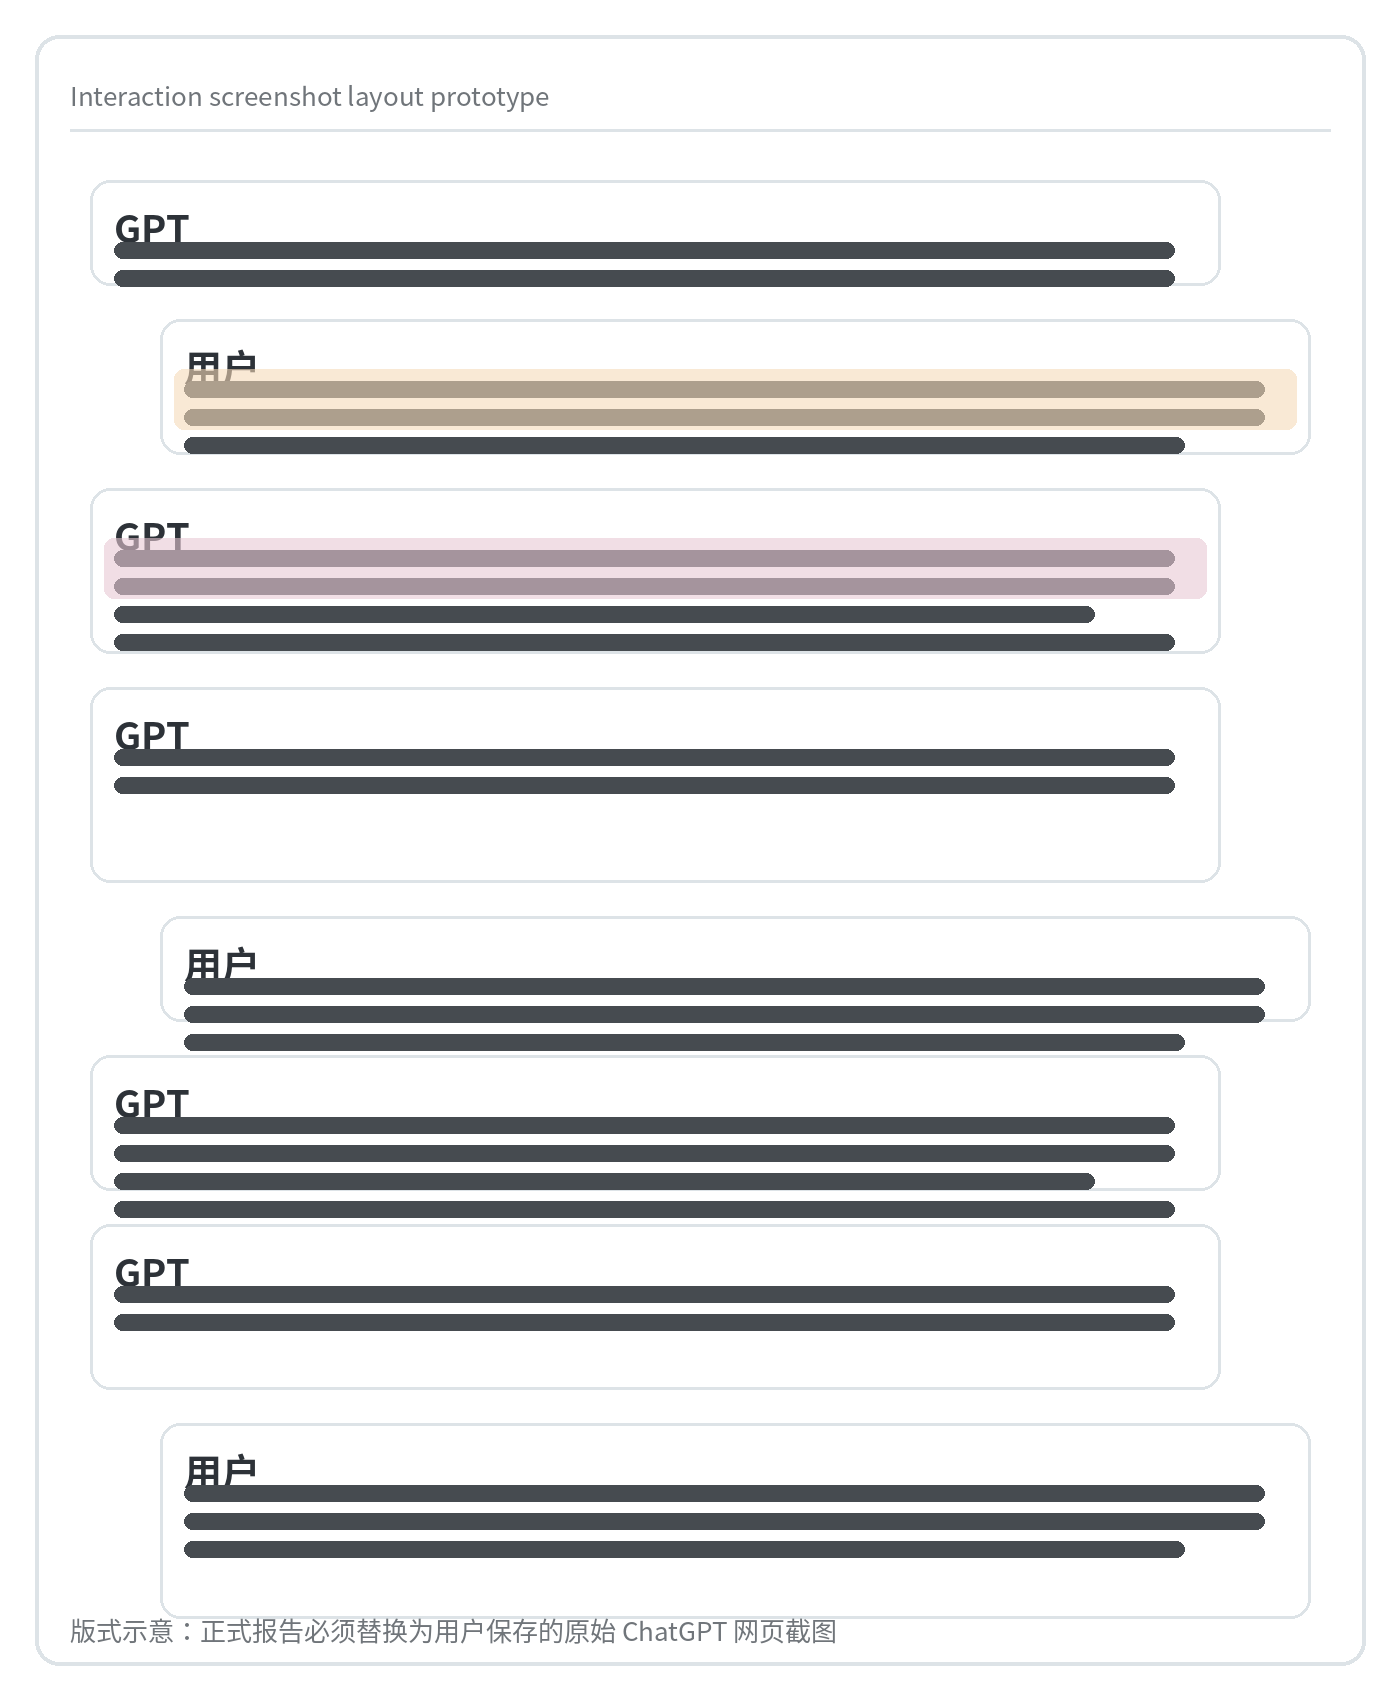
\includegraphics[
  width=\linewidth
]{demo-assets/interaction_part1.png}

\end{minipage}
\hfill
\begin{minipage}[t]{.28\linewidth}
\vspace{0pt}

\vspace{4mm}

\semantic{P2}{① 用户判断}

\par
\vspace{2mm}

用户指出原有方案隐含了一个未经验证的统一假设。

\par
\vspace{6mm}

\semantic{P3}{② 被质疑假设}

\par
\vspace{2mm}

需要把 AI 建议中的隐含前提单独拿出来验证。

\par
\vspace{6mm}

\semantic{P4}{③ 后续动作}

\par
\vspace{2mm}

如果讨论仍不能决定，就转为公平并行实验。

\end{minipage}

% ------------------------------------------------------------

\clearpage

\section*{核心交互：连续多页证据（2/3)}
\addcontentsline{toc}{section}{核心交互：连续多页证据（2/3）}

\begin{contextbox}
\textbf{SYNTHETIC / TEMPLATE ONLY}\par
连续页不机械重复固定两栏。

可根据原始截图比例使用宽幅截图，
并在上方、侧边或下方加入必要说明；

highlight、编号和箭头使用 P2 语义色，
但正文保持深灰。

批注解释证据价值，不重新编造聊天内容。
\end{contextbox}

\begin{figure}[H]
\centering

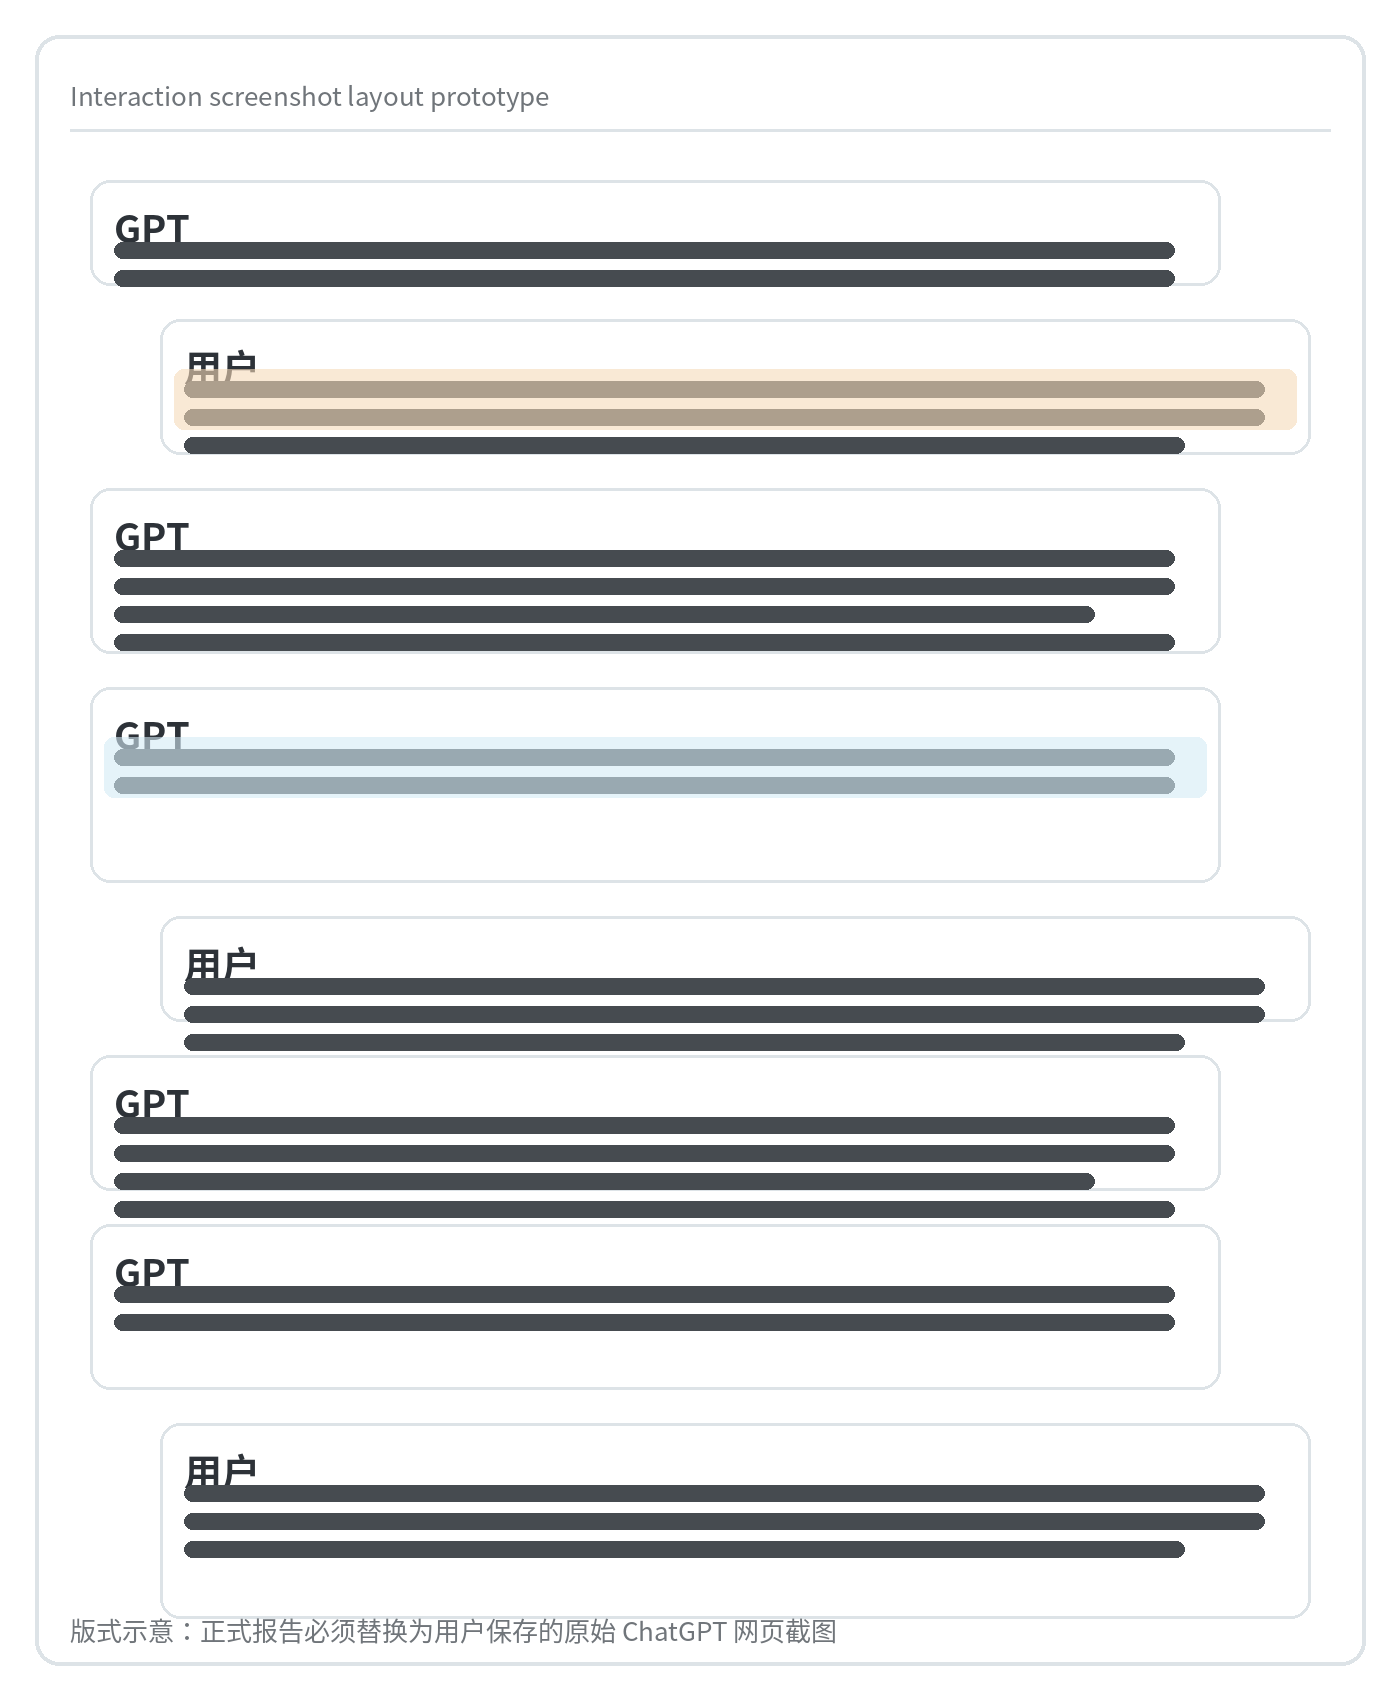
\includegraphics[
  width=.86\linewidth
]{demo-assets/interaction_part2.png}

\caption{
连续证据页示意。
正式版按消息边界裁切，
不从一条重要消息中间强行分页。
}
\end{figure}

\noindent
\semantic{P2}{用户建议}
\quad
把“统一参数”与“分类参数”都保留为候选，
而不是直接冻结一个方案。

\par
\vspace{4mm}

\noindent
\semantic{P4}{GPT修正}
\quad
将原先单一路径改成公平对照实验设计，
并等待真实证据裁决。

% ------------------------------------------------------------

\clearpage

\section*{核心交互：连续多页证据（3/3）}
\addcontentsline{toc}{section}{核心交互：连续多页证据（3/3）}

\begin{figure}[H]
\centering

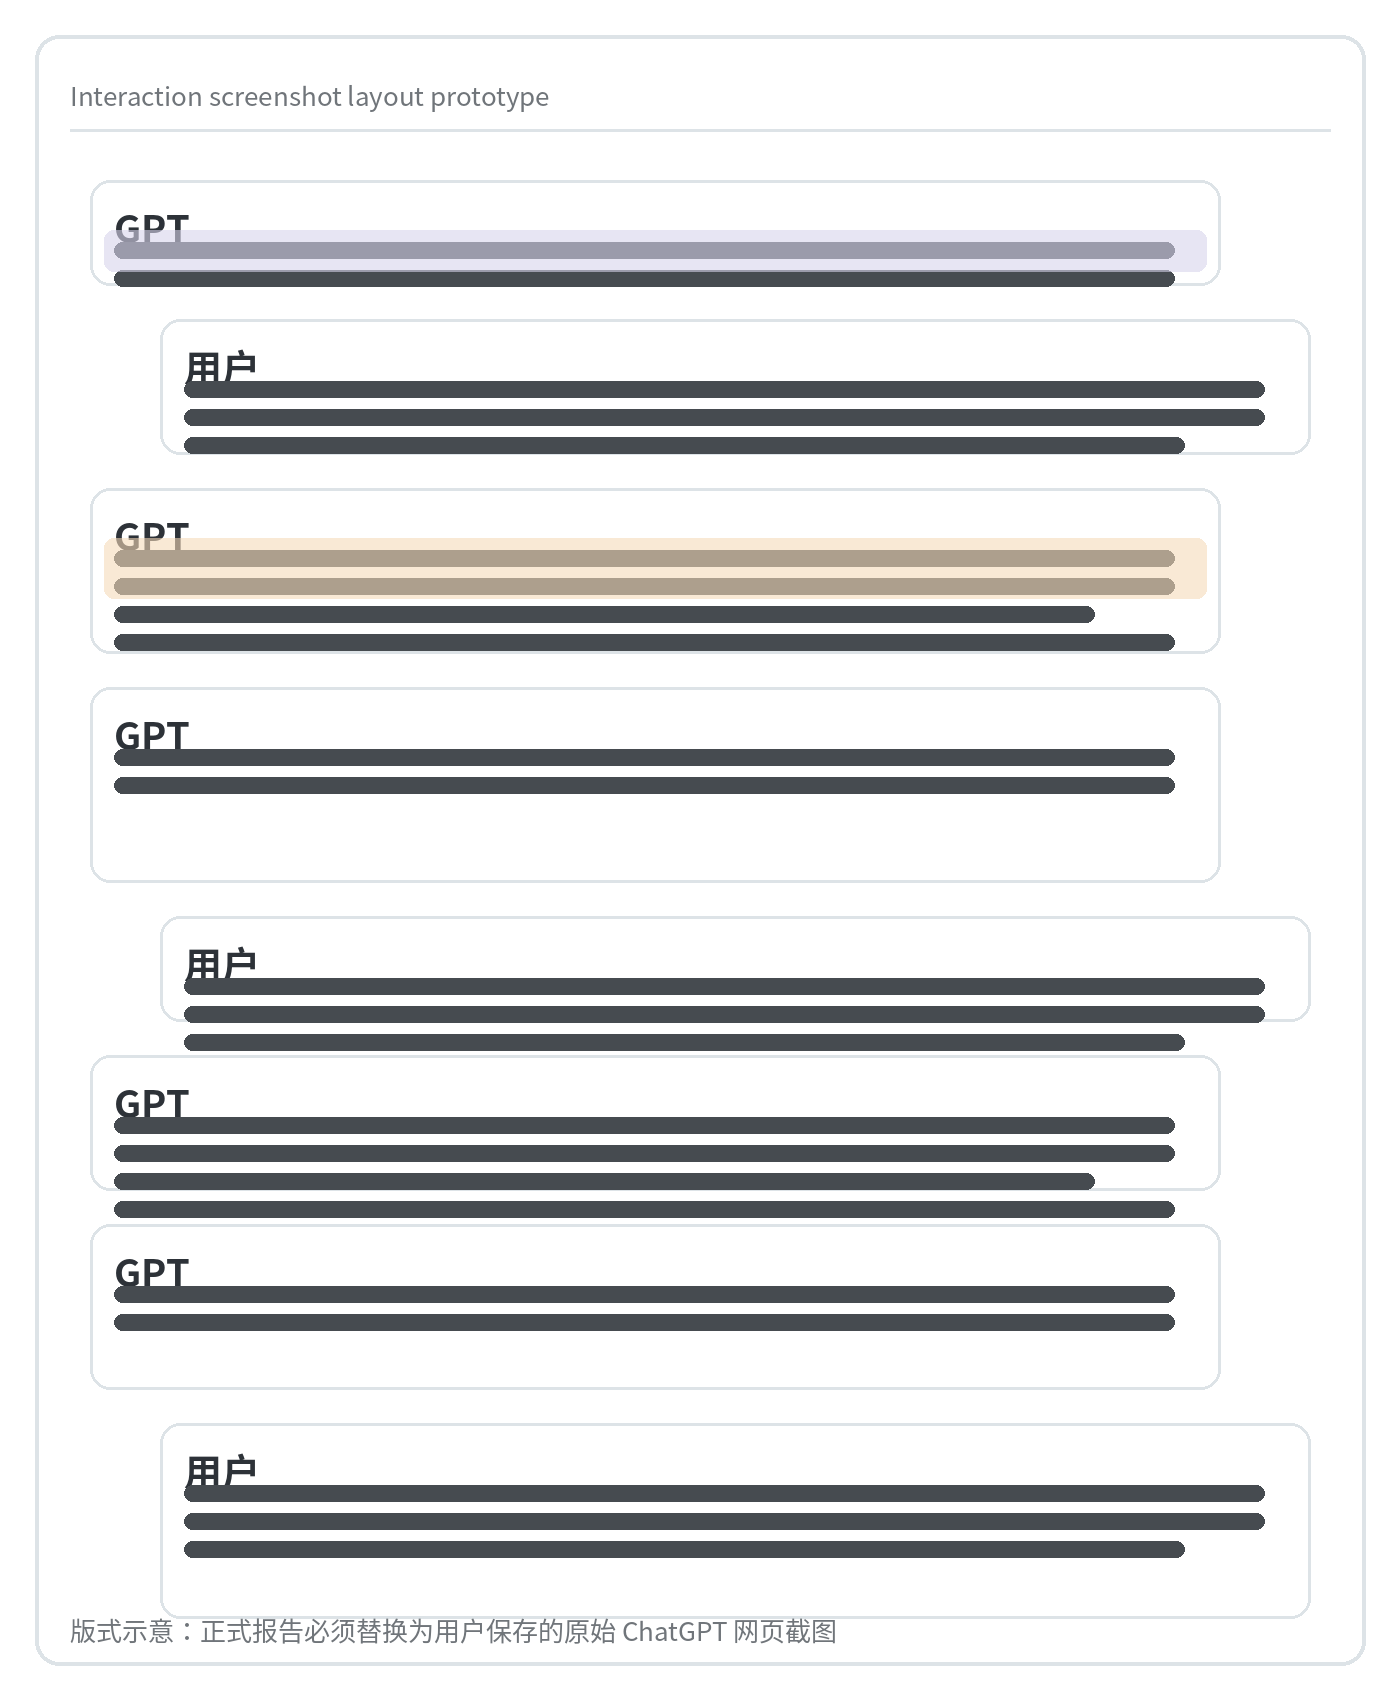
\includegraphics[
  width=.80\linewidth
]{demo-assets/interaction_part3.png}

\caption{
SYNTHETIC / TEMPLATE ONLY：核心交互收尾页示意。
正式版本必须替换为真实最终确认。
}
\end{figure}

\begin{decisionbox}[C4]
\textbf{最终确认必须保留。}

关键决策不仅展示讨论过程，
还应保留真实的最终确认截图，
并明确写出：

“最终决定是什么、依据是什么、下一步是什么”。

后续阶段性复盘必须标注为
当前对真实历史的总结与确认，
不能冒充原始对话。
\end{decisionbox}

% ============================================================
% 4. Human reasoning
% ============================================================

\clearpage

\section{用户思考、证据与最终决定}

\begin{contextbox}
这是 Process Report 最重要的图型之一，
可用于 Workflow Construction
或 Experiment Decision Process。

具体展示：

用户根据什么发现问题、
如何形成判断、
提出什么建议、
用什么资料 / 数据 / 实验验证，
以及最后怎样决定。

GPT 建议可以提供背景，
但不能掩盖人的真实推理链。
\end{contextbox}

\begin{figure}[H]
\centering

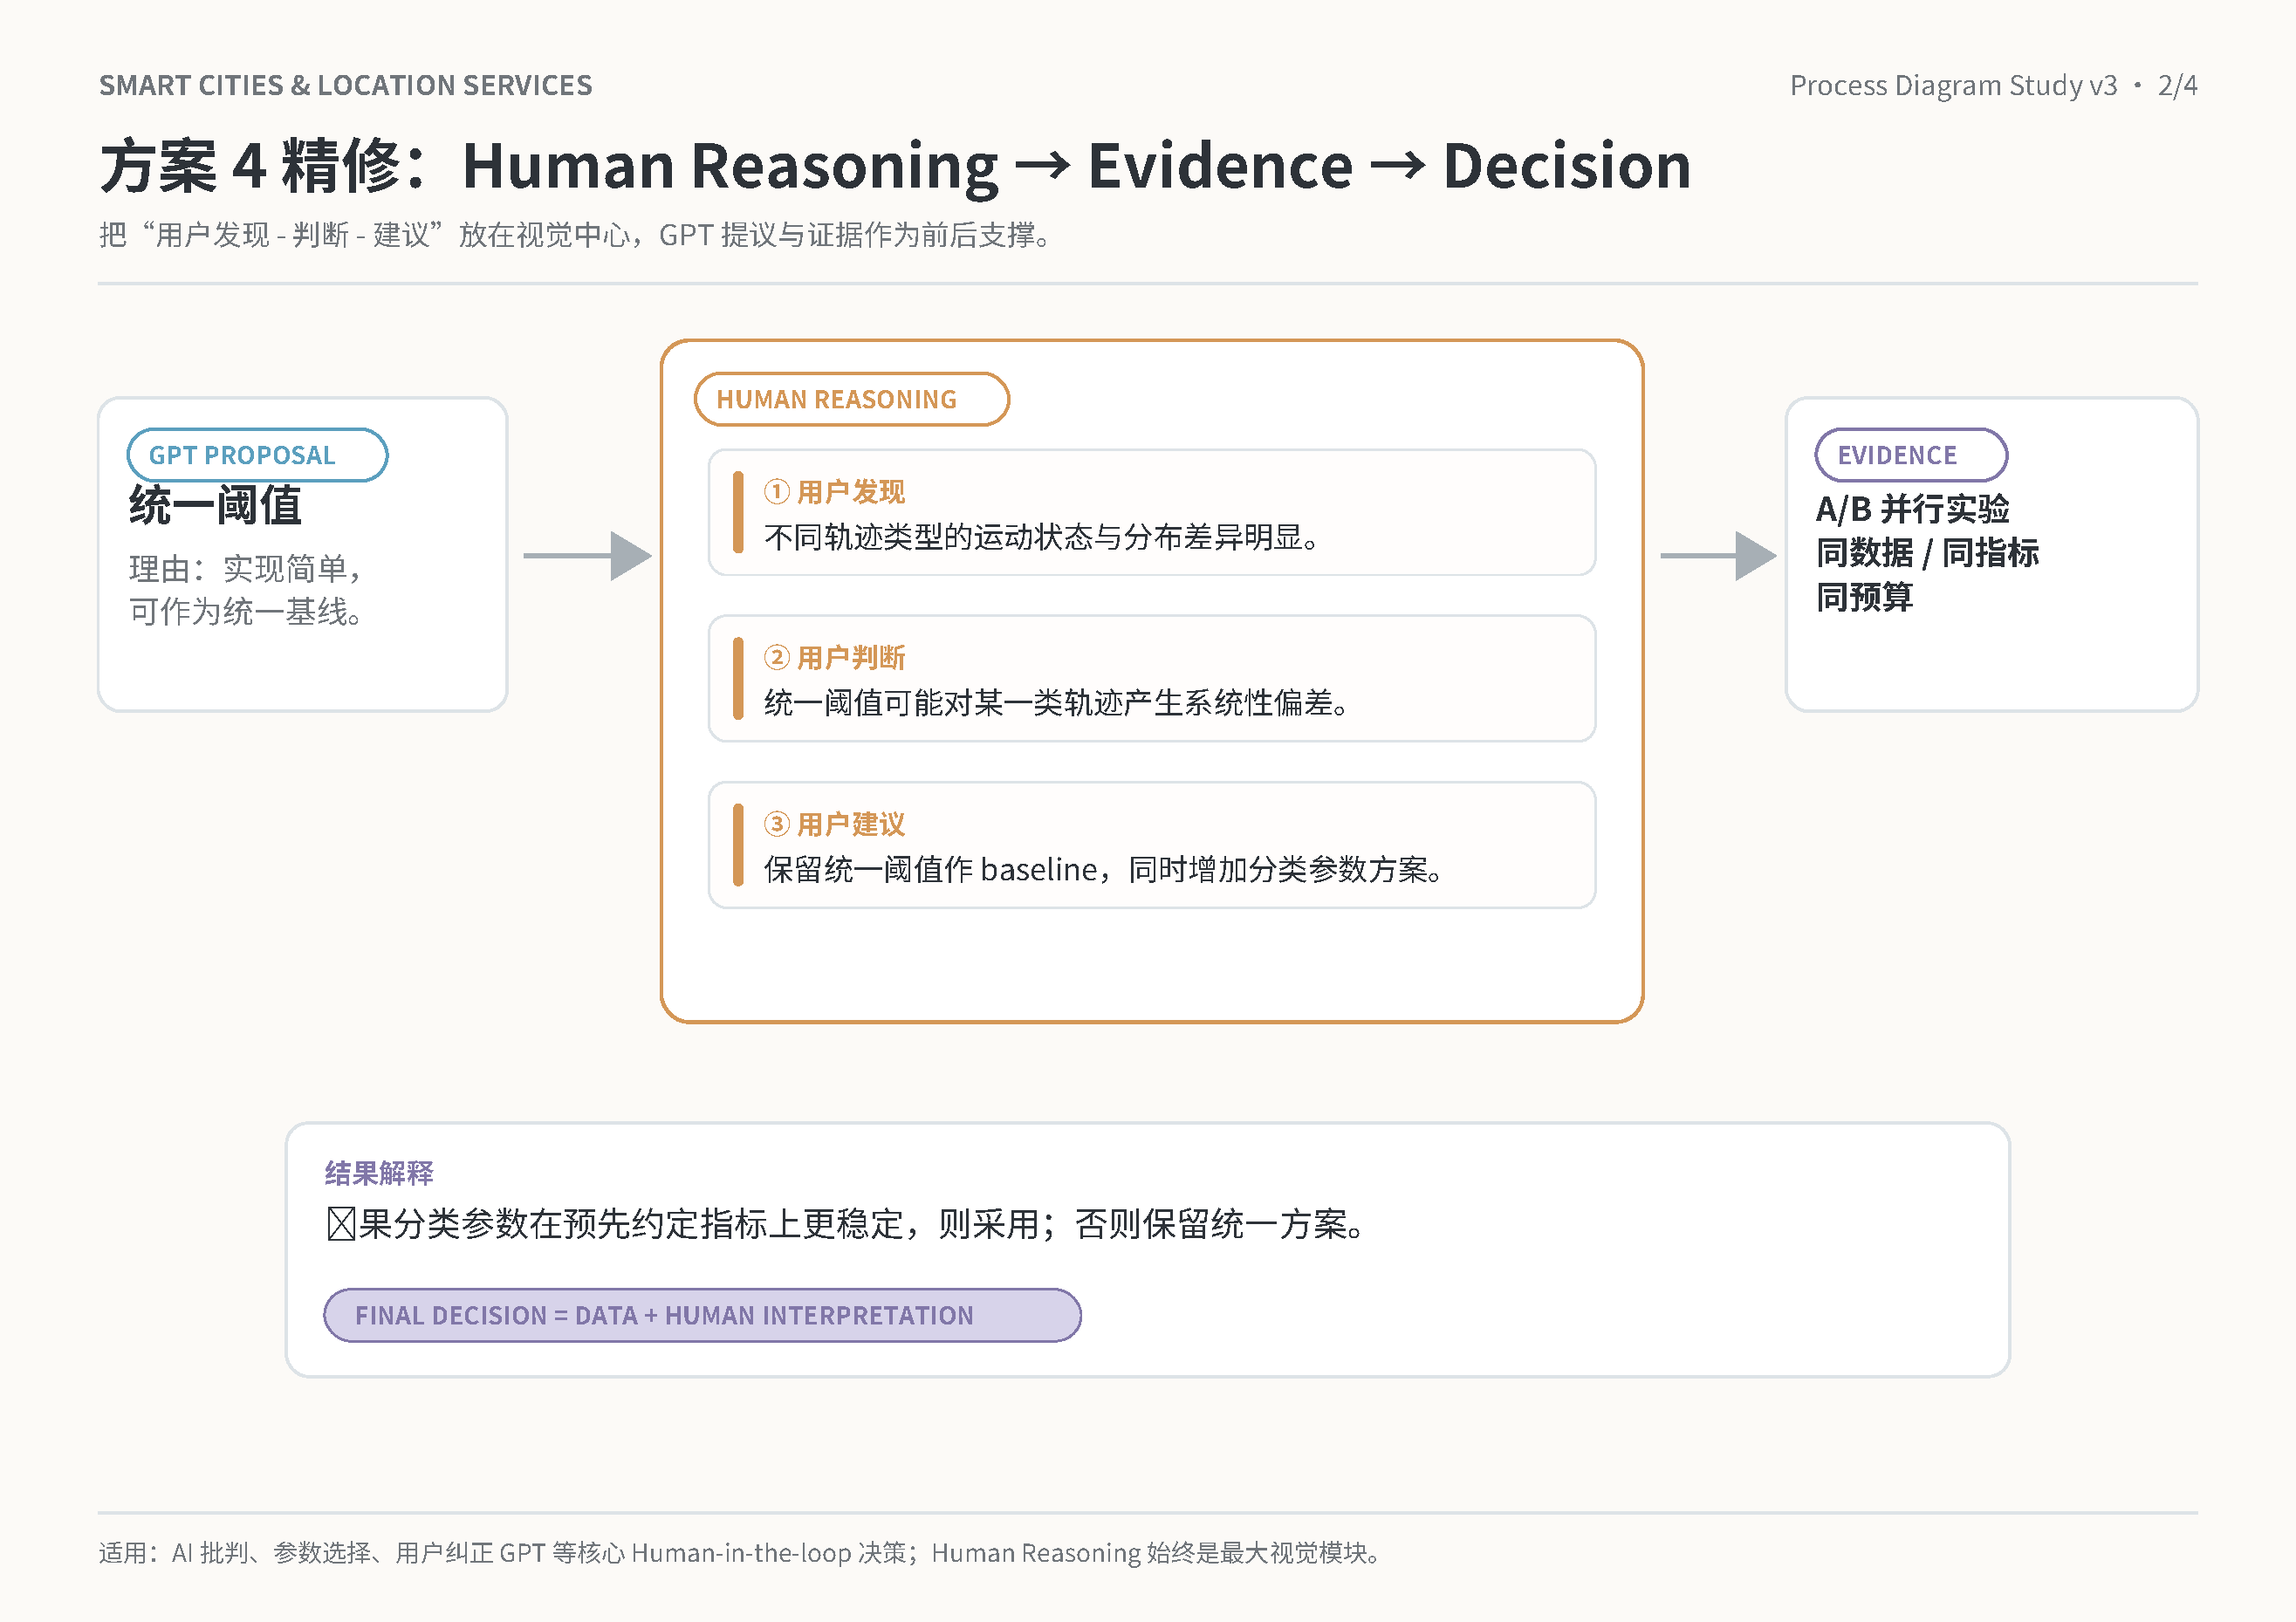
\includegraphics[
  width=.96\linewidth
]{demo-assets/human_reasoning.pdf}

\caption{
Human Reasoning → Evidence → Decision。
正式内容必须来自真实对话、资料、数据或实验。
}
\end{figure}

% ============================================================
% 5. Candidate decision tree
% ============================================================

\clearpage

\section{多候选方案如何筛选}

\begin{contextbox}
当一个问题存在多个实质候选时，
使用横向 Candidate Decision Tree 表达：

“保留、修改、测试、搁置、淘汰、进入并行实验”

的逻辑。

候选可以是：

实验方法、参数、指标，

也可以是：

工作流机制或正式产物结构。

颜色只做小范围语义标记，
普通节点保持白底。
\end{contextbox}

\begin{figure}[H]
\centering

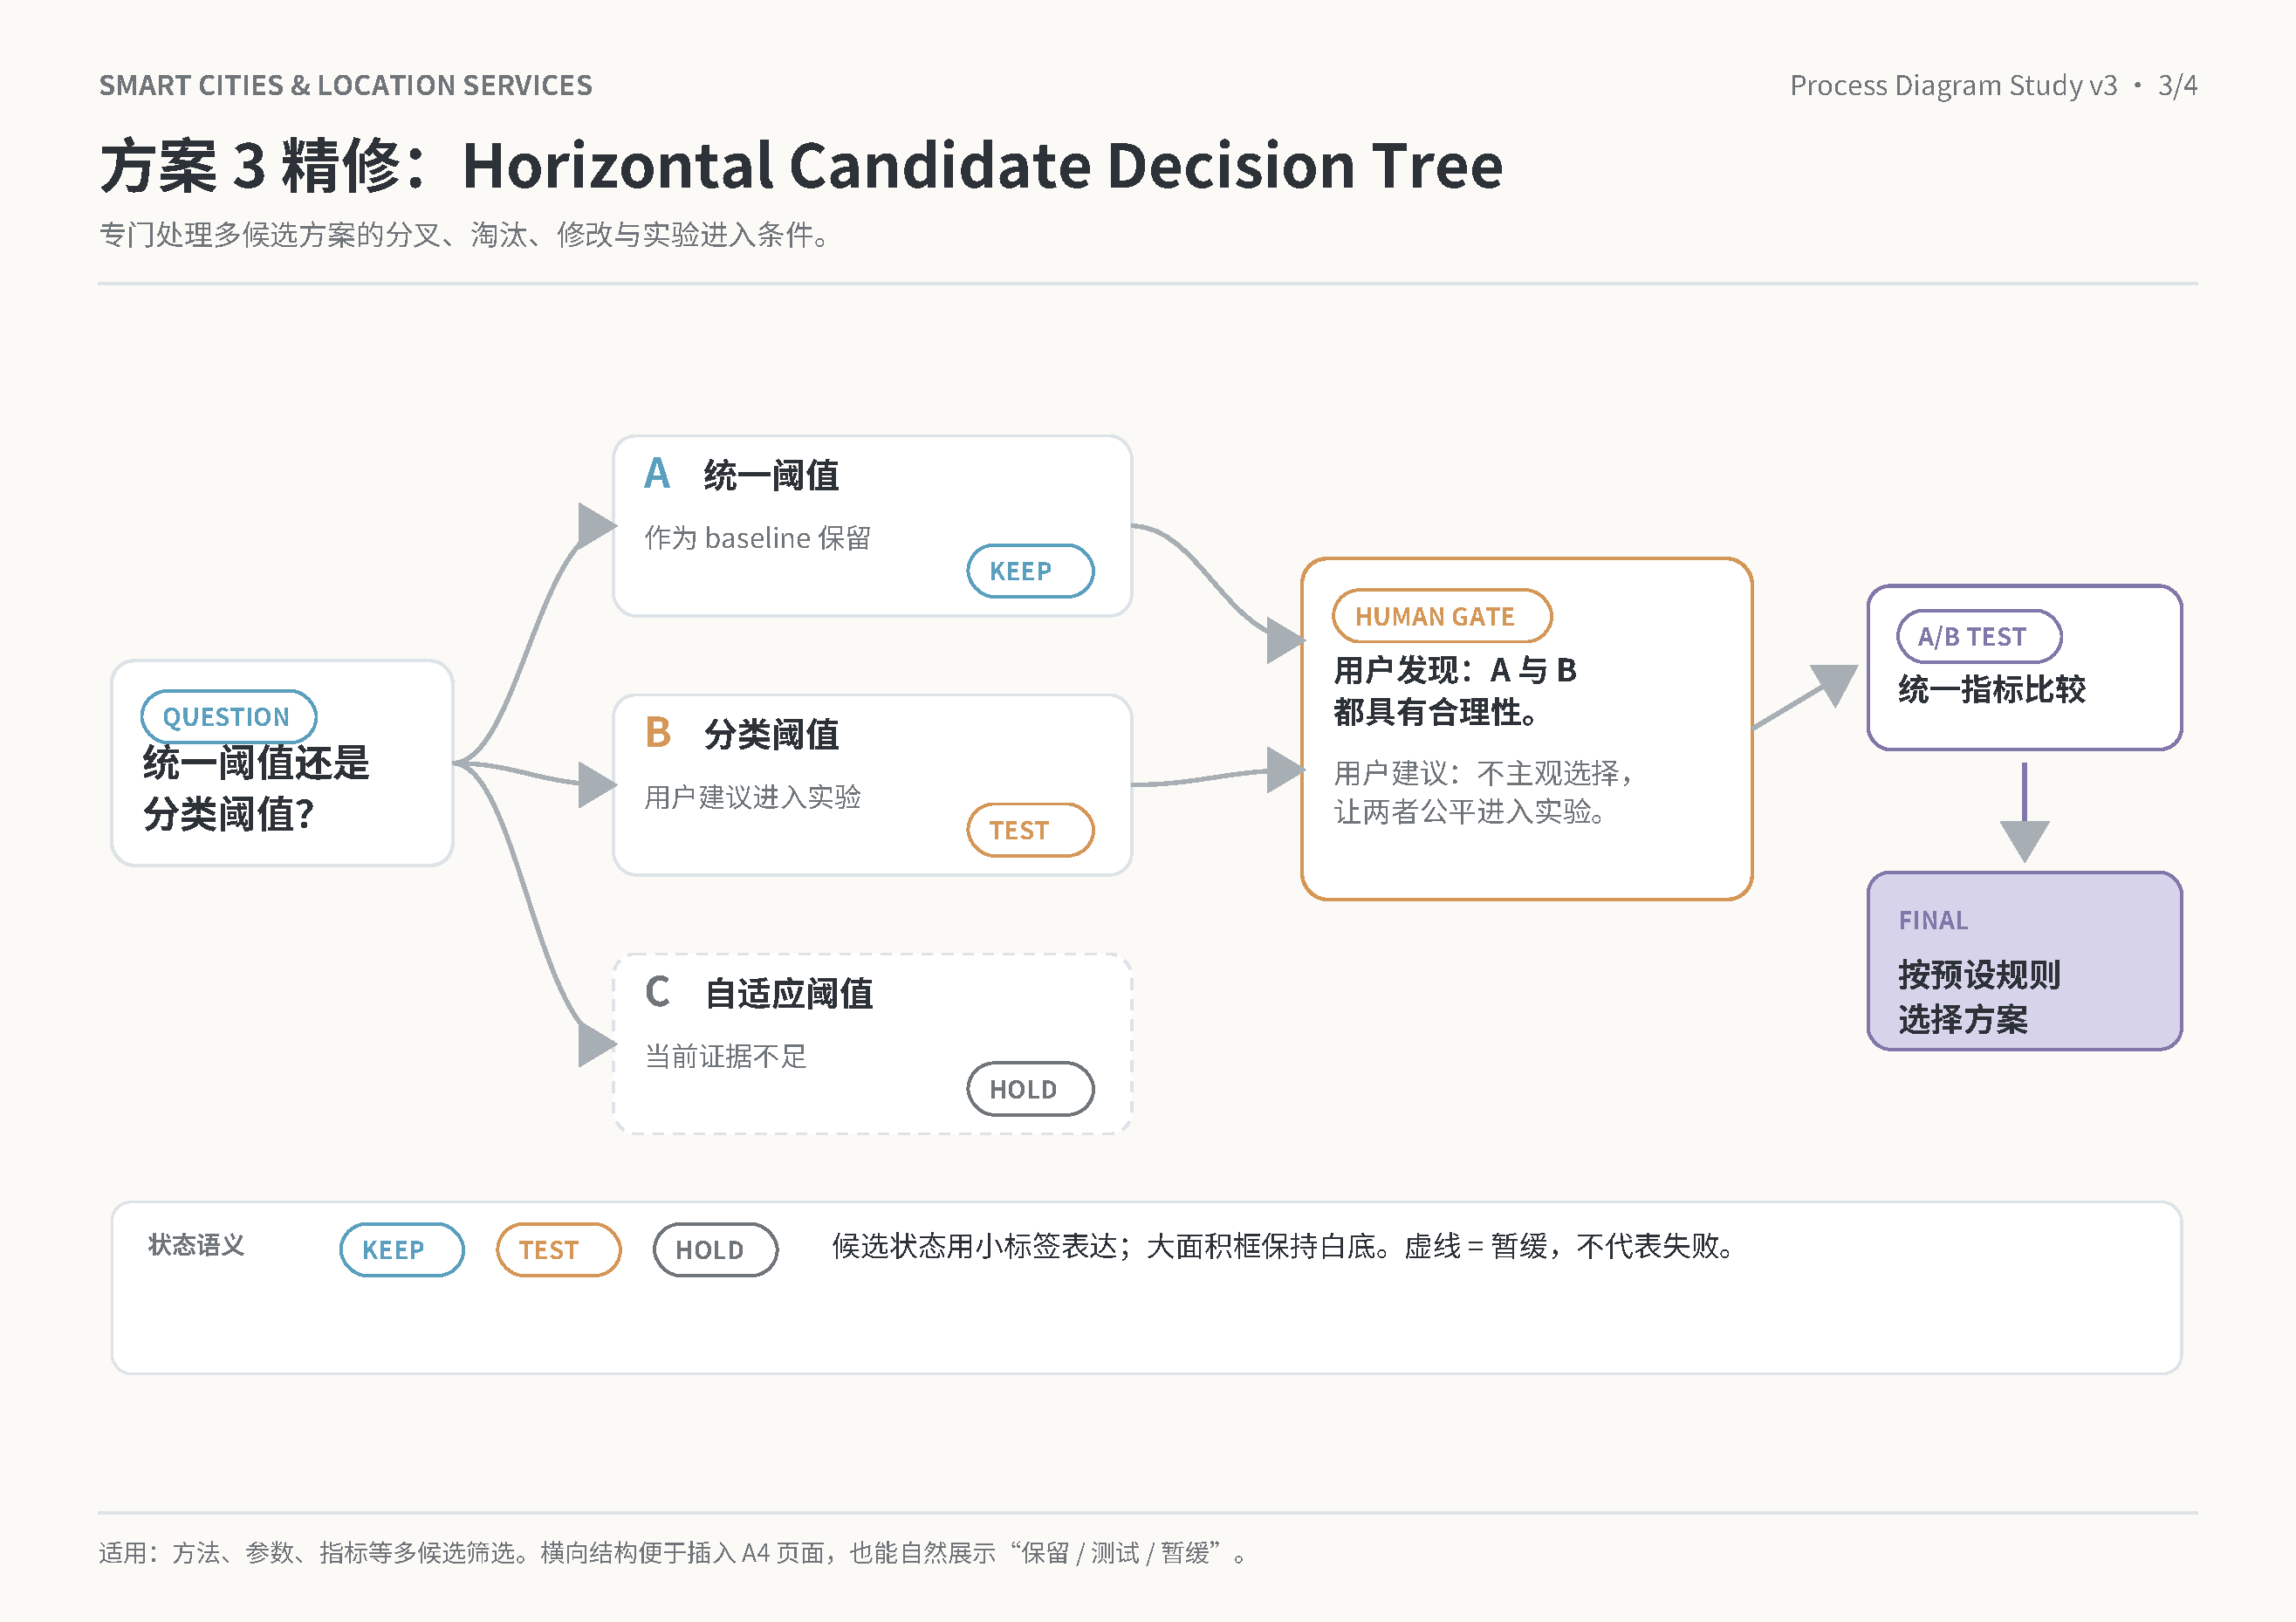
\includegraphics[
  width=.96\linewidth
]{demo-assets/candidate_tree.pdf}

\caption{
Horizontal Candidate Decision Tree。
正式版本应标明候选为何进入
KEEP / MODIFY / TEST / HOLD / REJECT
或最终选择。
}
\end{figure}

% ============================================================
% 6. Editorial summary
% ============================================================

\clearpage

\section{阶段性总结与下一轮研究}

\begin{contextbox}
Editorial Decision Board 用于阶段总结：

背景、
用户关键判断、
技术 / 资料证据、
下一步

保持在一页内，
但不承担复杂分支。

它可总结工作流构建阶段，
也可总结具体实验阶段，

与 Human Reasoning 图
和 Candidate Tree
共同构成 Process Diagram Language。
\end{contextbox}

\begin{figure}[H]
\centering

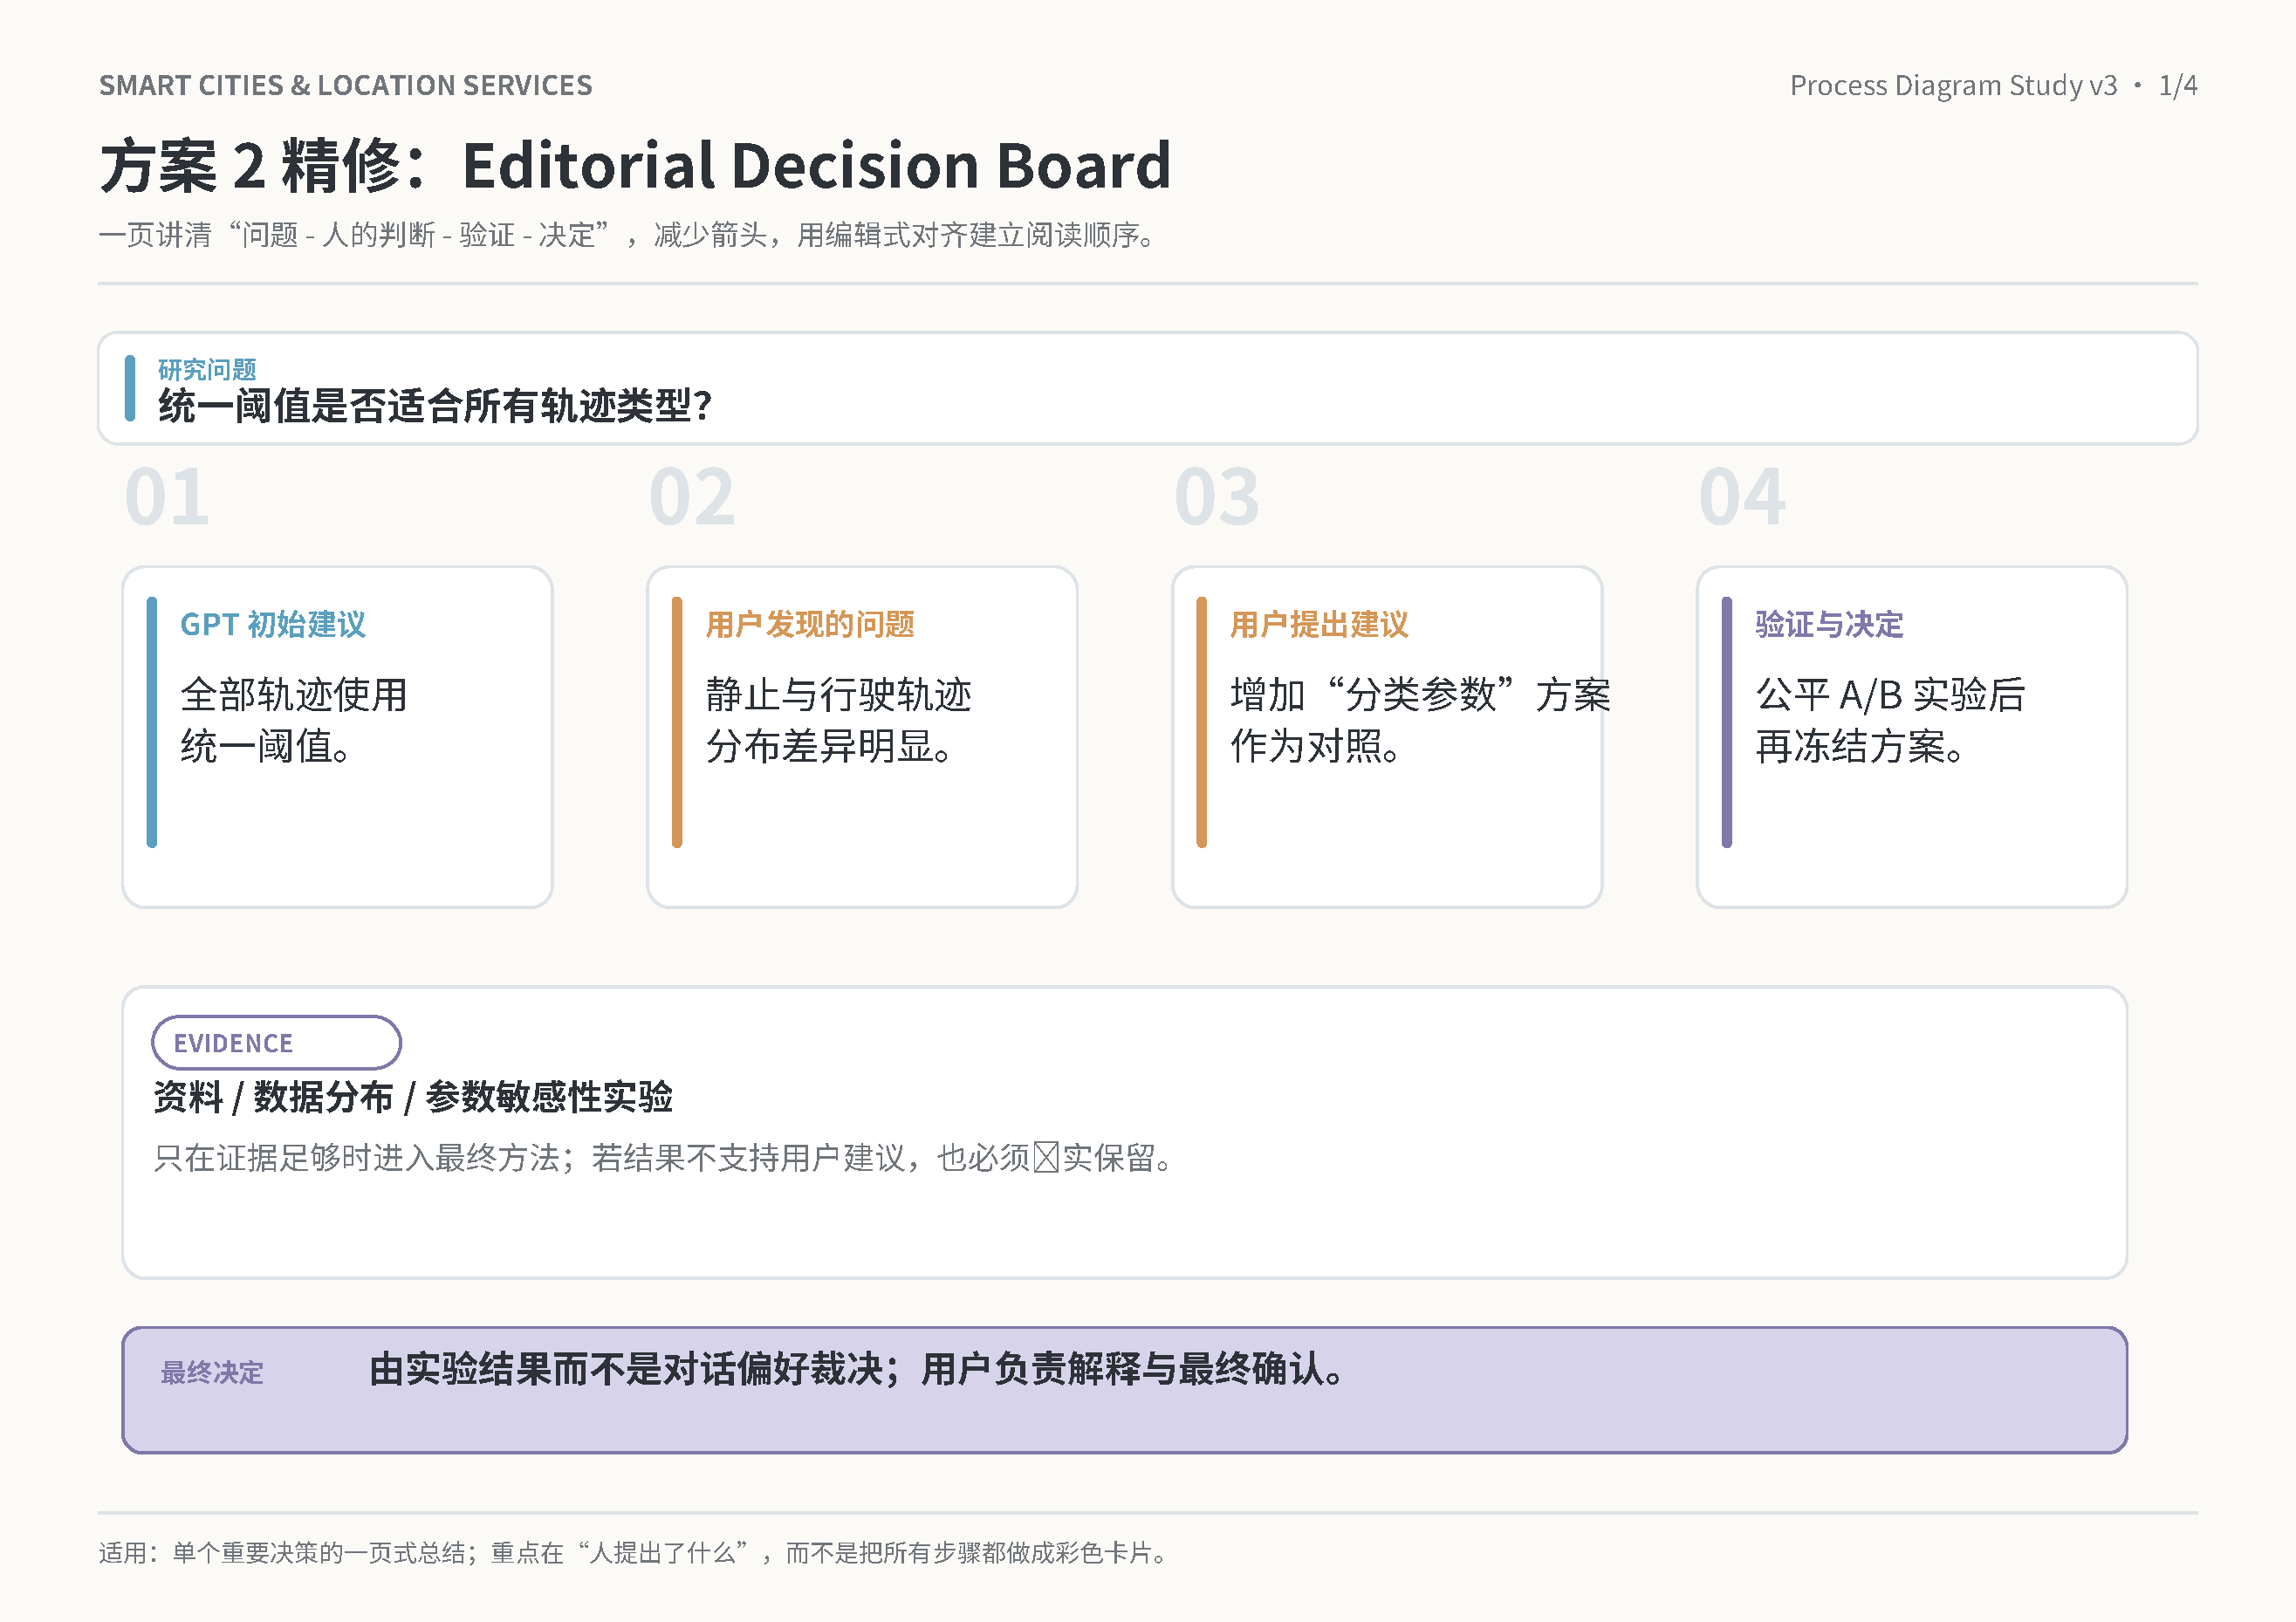
\includegraphics[
  width=.94\linewidth
]{demo-assets/editorial_board.pdf}

\caption{
Editorial Decision Board。
}
\end{figure}

\begin{decisionbox}[C4]
\textbf{Process Report 的核心证据循环：}

\quad
Idea
→ Interaction
→ Human Judgment
→ Evidence
→ Decision。

一般过程汇总展示，
关键过程展开，
最终确认保留。

判断内容是否进入正式报告的核心标准是：

\textbf{是否具有真实决策价值}

而不是它属于实验、GitHub、视觉系统
还是其他工作流模块。
\end{decisionbox}

% ============================================================
% 7. Usage boundary
% ============================================================

\section{使用边界}

本模板锁定的是视觉语言和证据组织方式，
不锁死具体章节名、页数或每类证据数量。

正式任务中，
只使用真实任务、真实资料、
真实交互、真实实验和真实决定
替换示例内容。

Process Report 负责两件事：

第一，
说明可靠 Human--AI 工作流如何形成；

第二，
说明具体研究决策如何形成。

具有实质决策价值的：

- 角色分工；
- Source Audit；
- T1--T4；
- UNRESOLVED 机制；
- Human--AI Evidence；
- 两份报告体系；
- Visual System；
- publication-plots 接入；
- GitHub Full Mirror；
- Submission Package 分离；

都可以进入 Workflow Construction。

但：

- 缓存删除；
- Zone.Identifier 清理；
- 普通路径修复；
- 无意义 Debug；
- 临时编译 housekeeping；

通常只保留在 internal evidence。

Experiment Report 负责说明：

最终方法是什么、
实验如何完成、
结果意味着什么。

两份报告可以共享同一真实事实来源，
但不得机械复制：

- 同一张 Brainstorm；
- 同一段聊天；
- 同一幅 Process Diagram。

\end{document}